%\documentclass[iop]{emulateapj}
%\documentclass[12pt, preprint]{emulateapj}
\documentclass[12pt, onecolumn]{emulateapj}

\usepackage{amsmath}
%\usepackage{bibtex}
%\bibliographystyle{unsrtnat}

\newcommand{\myemail}{aimalz@nyu.edu}
\newcommand{\textul}{\underline}
\newcommand{\scippr}{\texttt{scippr}}

%\slugcomment{}

\shorttitle{Probabilistic inference of the Hubble parameter}
\shortauthors{Malz and Peters, et al.}

\begin{document}

\title{Supernova Cosmology Inference with Probabilistic Photometric Redshifts}

\author{Alex Malz\altaffilmark{1}}
\author{Tina Peters\altaffilmark{2}}
\author{Humna Awan}
\author{Anita Bahmanyar\altaffilmark{2}}
\author{Lluis Galbany}
\author{Renee Hlozek\altaffilmark{2}}
\author{Boris Leistedt\altaffilmark{1}}
\author{Kara Ponder}
\altaffiltext{1}{Center for Cosmology and Particle Physics, Department of Physics, New York University, 726 Broadway, 9th floor, New York, NY 10003, USA}
\altaffiltext{2}{Dunlap Institute \& Department of Astronomy and Astrophysics, University of Toronto, 50 St George Street, Toronto, ON M5S 3H4 Canada}
\email{aimalz@nyu.edu}

\begin{abstract}
The BEAMS framework employs probabilistic supernova classifications to estimate the Hubble parameter that quantifies the relationship between distance and redshift over cosmic time.  This work extends BEAMS to replace high-confidence spectroscopic redshifts with probabilistic photometric redshifts, enabling inference of the Hubble parameter as a function of two probabilistic variables.  By combining posterior probabilities of supernova type and posterior probabilities of host galaxy redshift, we infer a posterior probability distribution over the redshift-dependent Hubble parameter.  This work also produces the \scippr code that can be used to infer cosmological parameters from probabilistic supernova fit parameters.
\end{abstract}

\keywords{}

\section{Introduction}
\label{sec:intro}

\citet{kunz_bayesian_2007, kelly_flexible_2008, hlozek_photometric_2012}

\begin{itemize}
	\item LSST era of photometric-only lightcurves and unreliable redshift point estimates
	\item BEAMS and type probabilities
	\item photo-$z$ PDFs
\end{itemize}

The problem at hand is to infer the cosmological parameters and redshift-dependent supernova type proportions from purely photometric data in the form of supernova lightcurves and host galaxy photometry.

\section{Method}
\label{sec:method}

This work demonstrates a principled approach to inferring cosmological parameters and redshift-dependent supernova type proportions from purely photometric lightcurves of supernovae and host galaxy photometry.  First, we outline the notation used throughout this paper.

Let us consider observations of $N$ supernovae $n$, each with a photometric lightcurve $\textul{\ell}_{n}$ and host galaxy photometry $\vec{f}_{n}$ comprised of fluxes, magnitudes, or colors.  When we conduct a photometric survey, not all supernovae in the universe will make it into our sample due to selection effects; we cannot include observations we did not make, nor do we include those with low confidence or insufficiently complete data.  These choices are quantified by nuisance parameters $\vec{\alpha}$ and $\vec{\beta}$ restricting the supernova lightcurves and host galaxy photometry respectively.  

We believe that every supernova has several intrinsic parameters that are not directly observable: a type $t_{n}$, a redshift $z_{n}$, and a distance modulus $\mu_{n}$.   Traditional methods estimate the values of these parameters from observed lightcurves and host galaxy photometry by assuming that the lightcurves and host galaxy photometry are random variables drawn from distributions that are functions of these unobservable parameters.
 
The unobservable parameters, however, are themselves random variables, with type being discrete and redshift and distance modulus being continuous, drawn from distributions that are functions of some hyperparameters.  When we use types, redshifts, and distance moduli to constrain the cosmological parameters and/or redshift-dependent type proportions, we make this very assumption.  As in traditional approaches, we seek to constrain the cosmological parameters comprising $\vec{\Omega}$, among them the Hubble parameter $H_{0}$ and matter density $\Omega_{0}$, and the redshift-dependent type proportions parametrized by $\textul{\phi}$ under some parametrization that need not be specified at this time.  The redshift-dependent type proportions can be thought of as probabilities over type and redshift $p(t, z | \textul{\phi})$.

\subsection{Model}
\label{sec:model}

We introduce a hierarchical Bayesian model for inferring the hyperparameters without estimating the unobservable parameters.  The directed acyclic graph of Fig. \ref{fig:pgm} shows the relationships between the variables discussed above.  We assume that the parameters associated with supernova $n$ and its host galaxy are statistically independent of the parameters associated with supernova $n'$ and its host galaxy.

\vspace{1in}
\begin{figure}
\begin{center}
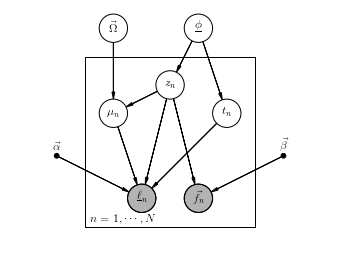
\includegraphics{fig/pgm.png}
\caption{This directed acyclic graph corresponds to a probabilistic graphical model for our hierarchical inference of the cosmological parameters and redshift-dependent type proportion parameters.  In this graph, all random variables are shown in circles, with observed variables shown in shaded circles.  The box indicates that there are $N$ copies of the relationships between boxed parameters, each statistically independent of all others.  The hyperparameters we would like to infer are the cosmological parameters in $\vec{\Omega}$ and the redshift-dependent type proportion parameters comprising $\textul{\phi}$.  Drawn from functions of these hyperparameters are the distance moduli $\{\mu_{n}\}_{N}$, redshifts $\{z_{n}\}_{N}$, and supernova types $\{t_{n}\}_{N}$.  Here, we observe host galaxy colors $\{\vec{f}_{n}\}_{N}$ and multi-band supernova lightcurves $\{\textul{\ell}_{n}\}_{N}$, shown in shaded circles.  The solid dots indicate known constants that factor into the model; $\vec{\alpha}$ represents the parameters defining a selection function in the space of observed lightcurves, and $\vec{\beta}$ includes the parameters defining a selection function in the space of host galaxy photometry.  The arrows encode the relationships between variables, going from parameters defining probability distributions to variables drawn from those probability distributions.}
\label{fig:pgm}
\end{center}
\end{figure}
\vspace{1in}

The motivation for this approach is the existence of photo-$z$ PDFs and the anticipation of PDFs over lightcurve fit parameters.  Photo-$z$ PDFs are posterior probability distributions; we observe the host galaxy photometry $\vec{f}_{n}$ and learn something about the host galaxy redshift $z_{n}$.  The process by which we derive a relationship between the observed and unobserved parameters imprints its biases in the form of an interim prior that defines a global probability distribution over redshifts parametrized by $\vec{\theta}$.  The selection function also biases the posterior probability in the form of an interim prior parametrized by $\vec{\beta}$.  Thus photo-$z$ PDF is an interim posterior probability distribution $p(z_{n} | \vec{f}_{n}, \vec{\theta}, \vec{\beta})$.

We anticipate the production of lightcurve parameter PDFs, which will also be interim posterior probability distributions, but in a higher dimensional space.  As in the case of photo-$z$ PDFs, the observed multi-band lightcurves $\{\vec{\ell}_{n}\}_{N}$ inform us about the latent parameters of supernova types $\{t_{n}\}_{N}$, redshifts $\{z_{n}\}_{N}$, and distance moduli $\{\mu_{n}\}_{N}$.  The interim prior will be a probability distribution over $t$, $z$, and $\mu$ with known parameters comprising $\textul{\xi}$.  We will also have a lightcurve selection function of parameters $\vec{\alpha}$ that is another distribution over this three-dimensional space.  The overall interim posterior of the supernova lightcurve is then $p(t_{n}, z_{n}, \mu_{n} | \textul{\ell}_{n}, \textul{\xi}, \vec{\alpha})$.

\textbf{(@aimalz Discuss interim priors and selection functions in more detail here, or somewhere else?)}

The goal here is to constrain the posterior distribution $p(\vec{\Omega}, \textul{\phi} | \{\textul{\ell}_{n}\}_{N}, \{\vec{f}_{n}\}_{N})$ of the physically important hyperparameters in $\vec{\Omega}$ and $\textul{\phi}$ given a catalog of $N$ interim posterior distributions $p(t_{n}, z_{n}, \mu_{n} | \textul{\ell}_{n}, \textul{\xi}, \vec{\alpha})$ and another $N$ interim posterior distributions $p(z_{n} | \vec{f}_{n}, \vec{\theta}, \vec{\beta})$.  We will derive an expression for the posterior distribution over hyperparameters that we want to find in terms of the interim posteriors over latent parameters that are available to us.

We begin by expanding this in terms of Bayes' Rule.
\begin{align}
\label{eq:bayes}
p(\vec{\Omega}, \textul{\phi} | \{\textul{\ell}_{n}\}_{N}, \{\vec{f}_{n}\}_{N}) &\propto p(\vec{\Omega}, \textul{\phi})\ p(\{\textul{\ell}_{n}\}_{N}, \{\vec{f}_{n}\}_{N} | \vec{\Omega}, \textul{\phi})
\end{align}
In plain English we are saying that the posterior probability of a certain cosmology and redshift-dependent type proportions given some set of observed supernova lightcurves and host galaxy photometry is proportional to the product of a prior belief about the cosomological parameters and redshift-dependent type proportions and the likelihood of the lightcurves and host galaxy photometry given the cosmology and redshift-dependent type proportions.

Next, we invoke the statistical independence of the supernova parameters and observations; each set of $(t_{n'}, z_{n'}, \mu_{n'}, \textul{\ell}_{n'}, \vec{f}_{n'})$ is independent from all other parameters in $\bigcup_{n}(t_{n\neq n'}, z_{n\neq n'}, \mu_{n\neq n'}, \textul{\ell}_{n\neq n'}, \vec{f}_{n\neq n'})$.
\begin{align}
\label{eq:independence}
p(\{\textul{\ell}_{n}\}_{N}, \{\vec{f}_{n}\}_{N} | \vec{\Omega}, \textul{\phi}) &= \prod_{n}^{N}p(\textul{\ell}_{n}, \vec{f}_{n} | \vec{\Omega}, \textul{\phi})
\end{align}
This assumption is necessary for us to easily combine the contributions of individual supernovae to the likelihood of the whole survey of supernovae. Here we are saying the the likelihood of the set of lightcurves and fluxes is simply the product of each of the individual likelihoods.

Next, we invoke marginalization over the latent variables, as an alternative to point estimation thereof.
\begin{align}
\label{eq:marginalization}
p(\textul{\ell}_{n}, \vec{f}_{n} | \vec{\Omega}, \textul{\phi}) &= \iiint p(\textul{\ell}_{n}, \vec{f}_{n} | \mu_{n}, z_{n}, t_{n})\ p(\mu_{n}, z_{n}, t_{n} | \vec{\Omega}, \textul{\phi})\ d\mu_{n}\ dz_{n}\ dt_{n}
\end{align}
This is how the unobservable variables enter the inference.  We note that Eq. \ref{eq:marginalization} calls for likelihoods $\{p(\textul{\ell}_{n}, \vec{f}_{n} | \mu_{n}, z_{n}, t_{n})\}_{N}$ of a supernova lightcurve and host galaxy photometry given some particular values of distance modulus, redshift, and type, but what we have are interim posteriors $\{p(\mu_{n}, z_{n}, t_{n} | \textul{\ell}_{n}, \vec{f}_{n}, \vec{\theta}, \textul{\xi}, \vec{\alpha}, \vec{\beta})\}_{N}$, which are probabilities of distance modulus, redshift, and type given set values for the supernova lightcurve, host galaxy photometry, and priors from the data analysis procedure and survey program.

We thus must transform our expression to be in terms of quantities we actually have.  We do this by multiplying the likelihood by an inspired factor of unity, in terms of the interim posteriors.
\begin{align}
\label{eq:unity}
p(\textul{\ell}_{n}, \vec{f}_{n} | \mu_{n}, z_{n}, t_{n}) &= p(\textul{\ell}_{n}, \vec{f}_{n} | \mu_{n}, z_{n}, t_{n})\ \frac{p(\mu_{n}, z_{n}, t_{n} | \textul{\ell}_{n}, \vec{f}_{n},\vec{\theta}, \textul{\xi}, \vec{\alpha}, \vec{\beta})}{p(\mu_{n}, z_{n}, t_{n} | \textul{\ell}_{n}, \vec{f}_{n}, \vec{\theta}, \textul{\xi}, \vec{\alpha}, \vec{\beta})}
\end{align}
We expand the denominator of that factor of unity according to Bayes' Rule.
\begin{align}
\label{eq:expand}
p(\textul{\ell}_{n}, \vec{f}_{n} | \mu_{n}, z_{n}, t_{n}) &= p(\textul{\ell}_{n}, \vec{f}_{n} | \mu_{n}, z_{n}, t_{n})\ \frac{p(\mu_{n}, z_{n}, t_{n} | \textul{\ell}_{n}, \vec{f}_{n},\vec{\theta}, \textul{\xi}, \vec{\alpha}, \vec{\beta})\ p(\textul{\ell}_{n}, \vec{f}_{n} | \vec{\theta}, \textul{\xi}, \vec{\alpha}, \vec{\beta})}{p(\mu_{n}, z_{n}, t_{n} | \vec{\theta}, \textul{\xi}, \vec{\alpha}, \vec{\beta})\ p(\textul{\ell}_{n}, \vec{f}_{n} | \mu_{n}, z_{n}, t_{n}, \vec{\theta}, \textul{\xi}, \vec{\alpha}, \vec{\beta})}
\end{align}
By the independence of the hierarchical levels in the probabilistic graphical model, we may split up the most daunting term in the above expression as
\begin{align}
\label{eq:breakdown}
p(\textul{\ell}_{n}, \vec{f}_{n} | \mu_{n}, z_{n}, t_{n}, \vec{\theta}, \textul{\xi}, \vec{\alpha}, \vec{\beta}) &= p(\textul{\ell}_{n}, \vec{f}_{n} | \mu_{n}, z_{n}, t_{n})\ p(\textul{\ell}_{n}, \vec{f}_{n} | \vec{\theta}, \textul{\xi}, \vec{\alpha}, \vec{\beta}).
\end{align}
Noting the presence of $p(\textul{\ell}_{n}, \vec{f}_{n} | \mu_{n}, z_{n}, t_{n})$ and $p(\textul{\ell}_{n}, \vec{f}_{n} | \vec{\theta}, \textul{\xi}, \vec{\alpha}, \vec{\beta})$ in both the numerator and denominator for $p(\textul{\ell}_{n}, \vec{f}_{n} | \mu_{n}, z_{n}, t_{n})$, we cancel the like terms to express the individual likelihoods in terms of known quantities, obtaining
\begin{align}
\label{eq:cancellation}
p(\textul{\ell}_{n}, \vec{f}_{n} | \mu_{n}, z_{n}, t_{n}) &= \frac{p(\mu_{n}, z_{n}, t_{n} | \textul{\ell}_{n}, \vec{f}_{n}, \vec{\theta}, \textul{\xi}, \vec{\alpha}, \vec{\beta})}{p(\mu_{n}, z_{n}, t_{n} | \vec{\theta}, \textul{\xi}, \vec{\alpha}, \vec{\beta})}.
\end{align}
We are now ready to plug the individual likelihoods into Eq. \ref{eq:marginalization}, leading to
\begin{align}
\label{eq:buildup}
p(\textul{\ell}_{n}, \vec{f}_{n} | \vec{\theta}, \textul{\phi}) &= \iiint p(\mu_{n}, z_{n}, t_{n} | \textul{\ell}_{n}, \vec{f}_{n}, \vec{\theta}^{*}, \textul{\phi}^{*})\ \frac{p(\mu_{n}, z_{n}, t_{n} | \vec{\theta}, \textul{\phi})}{p(\mu_{n}, z_{n}, t_{n} | \vec{\theta}^{*}, \textul{\phi}^{*})}\ d\mu_{n}\ dz_{n}\ dt_{n}
\end{align}
Finally, we plug Eq. \ref{eq:buildup} back into Eq. \ref{eq:independence}.
\begin{align}
\label{eq:plugin}
p(\{\textul{\ell}_{n}, \vec{f}_{n}\}_{N} | \vec{\Omega}, \textul{\phi}) &= \prod_{n}^{N}\ \iiint p(\mu_{n}, z_{n}, t_{n} | \textul{\ell}_{n}, \vec{f}_{n}, \vec{\theta}, \textul{\xi}, \vec{\alpha}, \vec{\beta})\ \frac{p(\mu_{n}, z_{n}, t_{n} | \vec{\Omega}, \textul{\phi})}{p(\mu_{n}, z_{n}, t_{n} | \vec{\theta}, \textul{\xi}, \vec{\alpha}, \vec{\beta})}\ d\mu_{n}\ dz_{n}\ dt_{n}
\end{align}
And finally, we plug the product back into Eq. \ref{eq:bayes} to obtain
\begin{align}
\label{eq:wrapup}
p(\vec{\Omega}, \textul{\phi} | \{\textul{\ell}_{n}, \vec{f}_{n}\}_{N}) &\propto p(\vec{\Omega}, \textul{\phi})\ \prod_{n}^{N}\ \iiint p(\mu_{n}, z_{n}, t_{n} | \textul{\ell}_{n}, \vec{f}_{n}, \vec{\theta}, \textul{\xi}, \vec{\alpha}, \vec{\beta})\ \frac{p(\mu_{n}, z_{n}, t_{n} | \vec{\Omega}, \textul{\phi})}{p(\mu_{n}, z_{n}, t_{n} | \vec{\theta}, \textul{\xi}, \vec{\alpha}, \vec{\beta})}\ d\mu_{n}\ dz_{n}\ dt_{n},
\end{align}
the posterior on cosmological parameters and redshift-dependent type proportions that we wish to sample.

It is very important to document the assumptions we make with this model:
\begin{enumerate}
	\item\label{it:completeness} The expression of Eq. \ref{eq:wrapup} is only as correct as the probabilistic graphical model of Fig. \ref{fig:pgm} is complete.
	\item\label{it:prior} We must choose a prior probability distribution $p(\vec{Omega}, \textul{\phi})$.
	\item\label{it:interimpriors} The interim prior parameters $\vec{\theta}$ and $\textul{\xi}$ are known and shared among all supernovae $n$.
	\item\label{it:selectionfunctions} The selection function parameters $\vec{\beta}$ and $\textul{\alpha}$ are known and shared among all supernovae $n$.
	\item\label{it:independence} All latent and observed parameters associated with the supernovae and their host galaxies are statistically independent from the latent and observed parameters of all other supernovae and their host galaxies.
	\item\label{it:accuracy} The interim posterior distributions $\{p(z_{n} | \vec{f}_{n}, \vec{\theta}, \vec{\beta})\}_{N}$ and $\{p(t_{n}, z_{n}, \mu_{n} | \textul{\ell}_{n}, \textul{\xi}, \vec{\alpha})\}_{N}$ are accurate.
\end{enumerate}
There are a few caveats to these assumptions.  

Item \ref{it:completeness} is present with any approach, as no model can include every aspect of the physics -- to make any problem tractable, we must make simplifications.  The hierarchical Bayesian approach, however, easily accommodates complications so is extensible to more refined models.

Skeptics of Bayesian statistics often cite item \ref{it:prior} as a major weakness of this approach.  It is true that choosing a prior distribution can impart a bias on the resulting inference, but it can be an advantage when the data quality is poor and there are already trustworthy constraints on the parameters in question.  We will nonetheless try to minimize the information imparted to the posterior by the prior.

It is noted that this model may be adapted to the cases when Items \ref{it:interimpriors} and \ref{it:selectionfunctions} are violated, which will be the case if the interim posteriors are not derived by a single method or if the photometry comes from a combination of surveys.  

Item \ref{it:independence} is never truly valid in that all data observed by a single instrument are correlated, for example, but if the data primarily inform us about the phenomenon in question and we believe the principle of the universality of physics, it is a safe assumption; furthermore, virtually no statistical analysis would be possible without it, so all alternative methods already make this assumption.

It may seem to go without saying, but Item \ref{it:accuracy} can be difficult to guarantee.  As will be discussed further in Sec. \ref{sec:data}, there is as yet no established method for producing the interim posterior distributions, and validating any such method's accuracy will be a challenge, as it has proven to be for photo-$z$ PDFs.

We implement the model of Sec. \ref{sec:model} in the form of the Supernova Cosmology Inference with Probabilistic Photometric Redshifts code \scippr, which is a \texttt{Python} code freely available to the community.

\section{Mock Data}
\label{sec:data}

The mock data used to validate this method is unusual in that joint interim posteriors over supernova type, redshift, and distance modulus have never before been made.  This paper does not approach the problem of how to produce this data product because doing so would require us to make many more assumptions that could limit the impact of this work.  As was mentioned in Sec. \ref{sec:model}, it is nontrivial to confirm the accuracy of any probabilistic data analysis method.  Doing so would require painstaking simulations of lightcurves and host galaxy photometry as well as a choice of lightcurve fitting scheme, and the method presented here would then depend on these being correct.  If the mock data consists of interim posteriors, we can verify their self-consistency with our knowledge of the selection functions and interim priors by way of a rigorous forward model.  For these reasons, we will assume that the data product in hand is a catalog of three-dimensional interim posteriors $\{p(\mu_{n}, z_{n}, t_{n} | \textul{\ell}_{n}, \vec{f}_{n}, \vec{\theta}, \textul{\phi}, \vec{\alpha}, \vec{\beta})\}_{N}$.

In this section, we outline the forward model by which the mock interim posteriors are generated.  The following subsections explain the choices made in our validation tests.  From this point on, we will only work with log-probability distributions

\subsection{The true hyperparameters and parameters}
\label{sec:true_hypers}

We begin by choosing parametrizations for the hyperparameters.  We must have some functions of the hyperparameters producing a distribution from which the supernova type, redshift, and distance modulus are drawn.  

For the redshift-dependent type proportions, we choose $p(t, z | \textul{\phi})$ to be a two-dimensional piecewise constant function over $T$ types and $Z$ redshift bins, making $\textul{\phi}$ a $T\times Z$ array with values $\phi_{i}$ equal to the probability of a supernova having the given type with a redshift in a given bin.  A normalization condition is enforced such that summing over the discrete variable of supernova type and integrating over all redshift bins yields a value of unity.  

To demonstrate that \scippr is an extension of BEAMS, we consider $T=3$, with $\tau\in\{Ia, Ibc, II\}$.  Under this parametrization, we use realistic values for the elements of $\textul{\phi}'$ derived by convolving the delay time distribution (DTD) and the star formation history.  This procedure is outlined in Secs. \ref{sec:TypeIaRate}, \ref{sec:TypeIbcRate}, and \ref{sec:TypeIIRate}.  As an overview, we set the relative rates of SN Ia and Core Collapse to be 25\% and 75\%, respectively, at z = 0.  \textbf{(@tinapeters How were these numbers modified for three SN populations?)}  We use the DTD for SN Ia from Graur et al (2013) and the DTD for SN II from Zapartas et al (2017), and the Cosmic Star Formation Rate from Behroozi et al (2013).  \textbf{(@tinapeters Put these references into the .bib file.)}  The redshift-dependent supernova type proportions derived in this way are shown in Fig. \ref{fig:relative_supernova_rates}.  \textbf{(@tinapeters What is the native format of these curves, i.e. a continuous function evaluated on a grid or something else?  I wrote about a piecewise constant function, but it can and should be whatever's consistent with the actual functions you calculated.)}  $N=10^{4}$ pairs of $(t'_{n}, z'_{n})$ are drawn from this distribution.

\begin{figure}
	\begin{center}
		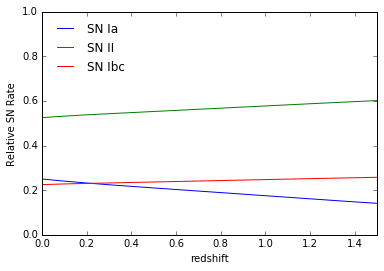
\includegraphics[width=0.5\textwidth]{fig/relative_supernova_rate.png}
		\caption{The relative supernova rates as a function of redshift. Sums to one at every redshift (but should actually integrate to one over type and redshift).  \textbf{(@aimalz Also plot the "observed" version of this for our sample)}}
		\label{fig:relative_supernova_rates}
	\end{center}
\end{figure}

For the parametrization of the cosmological parameters, we assume a $\Lambda$CDM cosmology so $\vec{\Omega}$ is comprised of $H_{0}$, $\Omega_{m}$, etc.  We choose the true cosmological parameters comprising $\vec{\Omega}'$ to be the maximum likelihood point estimates observed by Planck: $H_{0}=67.9\ Mpc/km/s$ and $\Omega_{m}=0.307$.  \textbf{(@aimalz fix these constants here and in code)}  The function that produces $\mu$ from a given $z_{n}$ is 
\begin{align}
\label{eq:distmod}
\mu &= 5\log\left[(1+z)\frac{1}{10\ pc}\int_{0}^{z}\frac{dz'}{\sqrt{\Omega_{M}(1+z)^{3}+\Omega_{k}(1+z)^{2}+\Omega_{\Lambda}}}\right].
\end{align}
This means that once the pair $(t'_{n}, z'_{n})$ is drawn from $p(t, z | \textul{\phi}')$, $p(\mu_{n} | \vec{\Omega}', z')$ is a delta function centered at $\mu'_{n}$ following Eq. \ref{eq:distmod}.  We have now set the true values of the hyperparameters and parameters
% $\textul{\phi}$ represents the parameters defining the supernova type proportions as a function of redshift, which we choose to be a $T\times Z$ dimensional matrix for a space with $T$ possible supernova types $\tau$ and $Z$ redshift bins $\zeta$ of widths $\vec{\Delta}_{z}$, where each element of $\phi_{\tau\zeta}$ is the probability density associated with a supernova of type $\tau$ with a redshift in bin $\zeta$; thus we have $p(z_{\zeta}, t_{\tau} | \textul{\phi}) \equiv \phi_{\zeta\tau}$, with $\textul{\phi}$ satisfying the normalization condition $\sum_{\tau=1}^{T}\textul{\phi}\cdot\vec{\Delta}_{z}=1$.  We proceed to choose a physically motivated true matrix of redshift-dependent supernova type proportions $\textul{\phi}'$.

\subsubsection{Supernova Type Ia Rate with Redshift}
\label{sec:TypeIaRate}

\subsubsection{Supernova Type Ibc Rate with Redshift}
\label{sec:TypeIbcRate}

\subsubsection{Supernova Type II Rate with Redshift}
\label{sec:TypeIIRate}

To determine the rate of SNII per unit comoving volume we will basically apply the approach by Forster et al. 2006/Strogler et al. 2004 adapted to SNe II following Botticella et al. 2012.

The rate of SNe II per unit time per unit comoving volume ($R_{II}$) is given by the star formation rate ($SFR$) per unit time per unit comoving volume convolved with the number of stars crearted that will explode as SNe II.

\begin{align}
	\label{eq:rateII_1}
	R_{II} = K_{II} \times SFR
\end{align}

First, we must calculate the fraction of stars that explode as SN II:

\begin{align}
\label{eq:rateII_2}
K_{II} = \frac{\int_{m_{l,II}}^{m_{u,II}} \phi(m) \mathrm{d}m}{\int_{m_{l}}^{m_{u}} m\phi(m) \mathrm{d}m}
\end{align}

When we integrate from a minimum mass, $m_{l,II}$, of 8 to a maximum mass, $m_{u,II}$, to 25 and assuming a Salpeter et al. (1955) IMF we get a rate of $6.027 \time 10^{-3}$.

We will use three different models of how the SFR evolutions with redshift: Cole et al. (2001), Horiuchi et al. (2011), and Madau et al. (2014)

\begin{figure}
	\begin{center}
		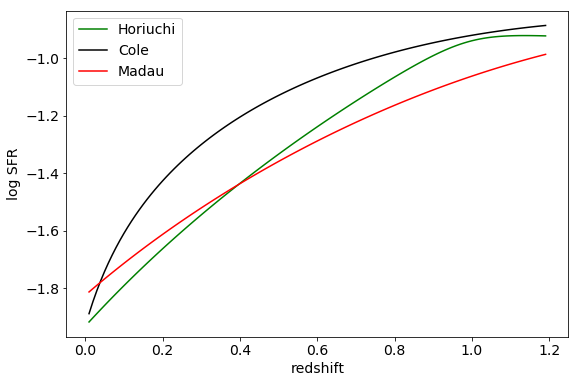
\includegraphics[width=0.5\textwidth]{fig/SNII_SFR.png}
		\caption{SFR evolutions with redshift: Cole et al. (2001), Horiuchi et al. (2011), and Madau et al. (2014).}
		\label{fig:SNII_SFR}
	\end{center}
\end{figure}

Next we will take the spectral model of Dessart et al. (2013) which is anchored to SN II 1999em, as a reference. We simulate its $r$-band light curve at different redshifts and convolve it with the LSST filters to see when it falls below the detection limit.

\begin{figure}
	\begin{center}
		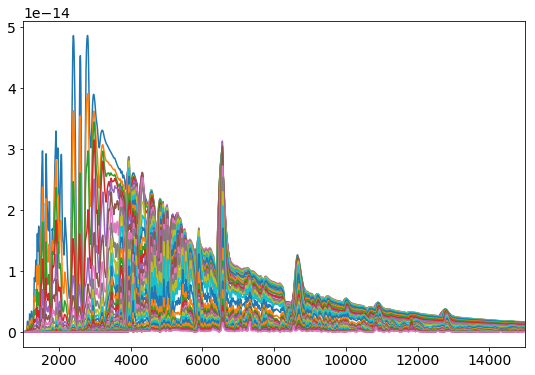
\includegraphics[width=0.5\textwidth]{fig/spectral_model_SNII.png}
		\caption{SN II spectral model of Dessart et al. (2013): $M_{99em}=-16.6$; $M_{05J}=-17.2$}
		\label{fig:SNII_lc}
	\end{center}
\end{figure}

\begin{figure}
	\begin{center}
		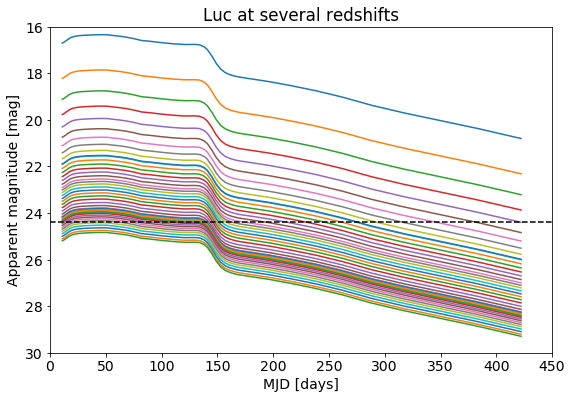
\includegraphics[width=0.5\textwidth]{fig/SNII_lc_withz.png}
		\caption{The $r$-band lightcurve of spectral model of SN II 1999em shifted to a range of redshifts. The horizontal dashed line indicates the limiting magnitude of LSST in the $r$-band in a single visit.}
		\label{fig:SNII_lc_withz}
	\end{center}
\end{figure}

For this model SN II, we compare the magnitude as a function of time and redshift, $m(t,z)$, with the limiting magnitude, $m_{lim}$, of the LSST camera to obtain the probability of detecting (the peak of) a SN at a given redshift, $\Delta_{t}(z)$. Then we estimate the number of detected SNe II per unit of redshift, $dN/dz$, using Equations 2 and 5 of Forster et al. (2006).

\begin{figure}
	\begin{center}
		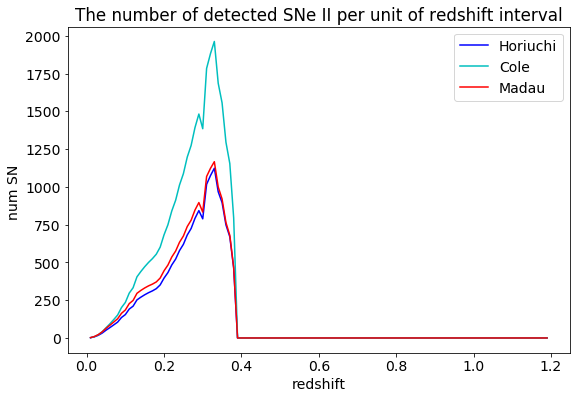
\includegraphics[width=0.5\textwidth]{fig/number_SNII.png}
		\caption{The number of SN II detected, for each of the SFR models, as a function of redshift. The total number of SN II for Horiuchi et al. 16985, Cole et al. 29207, and Madau et al.  18322. }
		\label{fig:SNII_lc_sfr}
	\end{center}
\end{figure}

Finally, we will use a a sample of 10,000 SNe, simulated using MCMC on real parameters of CSP SNe II. We will put each at 100 random redshifts from 0.01 to 1.20, so we will have 1,000,000 SNe. Now we consider the magnitude at the end of the plateau phase, instead of the peak magnitude. This is because in SN II cosmology, we do not standardize the magnitude at peak, but either the magnitude at around the center of the plateau (for spectroscopic methods), or the length/brightness-decline of the plateau (for photometric methods).

We use the apparent magnitudes at the end of the plateau phase and k-correct the magnitudes. Then we measure $\Delta_t(z)$, selecting different magnitude limit depending on the filter we use for observations. Finally, we compare the number of supernovae as a function of redshift for the three different SFR models.

\begin{figure}
	\begin{center}
		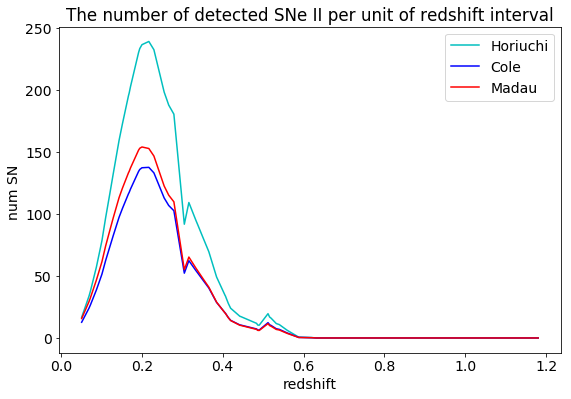
\includegraphics[width=0.5\textwidth]{fig/number_SNII_withmagntiudescatter.png}
		\caption{The number of SN II detected, for each of the SFR models, as a function of redshift. The total number of SN II for Horiuchi et al. 16985, Cole et al. 29207, and Madau et al.  18322. }
		\label{fig:SNII_lc_wz}
	\end{center}
\end{figure}
 
% \subsection{Setting true values of the latent variables}
% \label{sec:true_latents}
%
% To review, the latent variables are the supernova types $\{t_{n}\}_{N}$, redshifts $\{z_{n}\}_{N}$, and distance moduli $\{\mu_{n}\}_{N}$.  Now we must set a parametrization on the probability distributions $p(\mu_{n}, z_{n}, t_{n} | \textul{\ell}_{n}, \vec{f}_{n})$.  For the supernova type and redshift dimensions, we adopt the same parametrization used for $\textul{\phi}$.  There are $T$ supernova types and $Z$ redshift bins, indexed by $\tau$ and $\zeta$ respectively/  W, and $D$ bins in distance modulus indexed by $\nu$.  $\textul{\phi}$ describes 
%
% Because the redshift-dependent supernova type proportions are parametrized by $\textul{\phi}'$ such that $p(z\in\zeta, t=\tau | \textul{\phi}') = \phi_{\zeta\tau}$, it is easy to draw pairs of true types and redshifts $(t_{n}', z_{n}')$ from $\textul{\phi}'$.  We treat the elements of $\textul{\phi}'$ as a discrete distribution, noting that the redshift-dependent supernova type proportions are normalized such that $\sum_{\tau}\int_{\zeta}\textul{\phi}=1$.  Sampling the function defined by $\textul{\phi}'$ is equivalent to sampling true types and redshift bins.  Once the redshift bins have been chosen, we may choose a true redshift for each supernova from a uniform distribution defined between the bin endpoints.  This procedure gives us pairs of true types and redshifts $(t_{n}', z_{n}')$.
%
% Finally, we calculate the true $\mu_{n}'$ according to [insert distance modulus equation from astropy.cosmology here] from $z_{n}'$ and $\vec{\theta}'$.  Rather than writing the form of the distance modulus as a function of redshift and cosmological parameters throughout the paper, we will instead use the shorthand $\mu = f_{\vec{\theta}}(z)$ here.  This results in a true catalog of length $N$ consisting of trios $(t_{n}', z_{n}', \mu_{n}')$ of the latent variables.

\subsection{Constructing PDFs}
\label{sec:pdfs}

The catalog of trios of true latent variables must be transformed into three-dimensional probability distribution functions (PDFs) over these three variables.  To improve the efficiency of \scippr, we use a binned parametrization for the PDFs $p(\mu_{n}, z_{n}, t_{n} | \textul{\ell}_{n}, \vec{f}_{n}, \vec{\theta}, \textul{\xi}, \vec{\alpha}, \vec{\beta})$ so that the mathematical manipulations of the PDFs are simple operations on arrays.  This choice is made at the level of writing code, not something intrinsic to the model.  For these tests, we use $J=20$ equally spaced bins in redshift and $K=20$ equally spaced bins in distance modulus.  

We construct the PDFs from simple components described in the following sections, guided by the graphical model of Fig. \ref{fig:pgm}.  We will be assuming separability of the data 

% We will discuss the two terms separately. The first term of Eq. \ref{eq:mockBayes} may easily be reduced to $p(\textul{\ell}_{n}, \vec{m}_{n} | \mu_{n}, z_{n}, t_{n})$, as there is no direct dependence of the data on the hyperparameters.  Fig. \ref{fig:pgm} tells us how to break it up, resulting in Eq. \ref{eq:first}.
%
% \begin{align}
% \label{eq:first}
% p(\textul{\ell}_{n}, \vec{m}_{n} | \mu_{n}, z_{n}, t_{n}) &= p(\textul{\ell}_{n} | \mu_{n}, z_{n}, t_{n})\ p(\vec{m}_{n} | z_{n})
% \end{align}
%
% According to Fig. \ref{fig:pgm}, we have Eq. \ref{eq:second}.
%
% \begin{align}
% \label{eq:second}
% p(\mu_{n}, z_{n}, t_{n} | \vec{\theta}^{*}, \textul{\phi}^{*}) &= p(\mu_{n} | z_{n}, \vec{\theta}^{*})\ p(z_{n}, t_{n} | \textul{\phi}^{*})
% \end{align}
%
% These two terms will be addressed separately in Secs. \ref{sec:likelihoods} and \ref{sec:posteriors}.

\subsubsection{Creating posteriors}
\label{sec:posteriors}

The first components we must construct are the posterior distributions $p(\mu_{n}, z_{n}, t_{n} | \textul{\ell}_{n}, \vec{f}_{n})$.  We note the statistical independence of $\textul{\ell}_{n}$ and $\vec{f}_{n}$, as there are no direct connections between them in Fig. \ref{fig:pgm}.  Furthermore, while the supernova lightcurve is a function of all three latent variables, the host galaxy photometry is independent of the distance modulus and supernova type according to the model of Fig. \ref{fig:pgm}.  (Though there is some evidence against this assumption, the details of any potential relationship have not yet been determined well enough to model, so we do not include this effect at this time.)  Because of these instances of independence, we may decompose the posterior as
\begin{align}
\label{eq:posteriors_decompose}
p(\mu_{n}, z_{n}, t_{n} | \textul{\ell}_{n}, \vec{f}_{n}) &= p(\mu_{n}, z_{n}, t_{n} | \textul{\ell}_{n})\ p(z_{n} | \vec{f}_{n}).
\end{align}
We construct these terms without simulating supernova lightcurves nor host galaxy photometry.  The true supernova types, redshifts, and distance moduli serve as a proxy for the information that would be carried by the observed data; in other words, we are saying
\begin{align}
\label{eq:posteriors_emulate}
p(\mu_{n}, z_{n}, t_{n} | \textul{\ell}_{n}, \vec{f}_{n}) &= p(\mu_{n}, z_{n}, t_{n} | \mu'_{n}, z'_{n}, t'_{n})\ p(z_{n} | z'_{n}).
\end{align}
We thus emulate the desired posteriors based on our understanding of the forward model of point estimates of these quantities.

We first approach the second term, the photo-$z$ posterior.  The piecewise constant parametrization is flexible enough to accommodate many shapes for the redshift posterior, but for now, we assume it is a binned Gaussian distribution $\mathcal{N}(z_{n}''^{f}, \sigma_{f}^{2})$ with a variance $\sigma_{f}^{2}$ shared by the entire dataset and a mean of $z_{n}''^{f}$ drawn from a Gaussian distribution $\mathcal{N}(z'_{n}, \sigma_{f}^{2})$ of the same variance with a mean of $z'_{n}$, the true redshift.  Examples of these photo-$z$ posteriors are shown in Fig. \ref{fig:pzs}.

\begin{figure}
	\begin{center}
		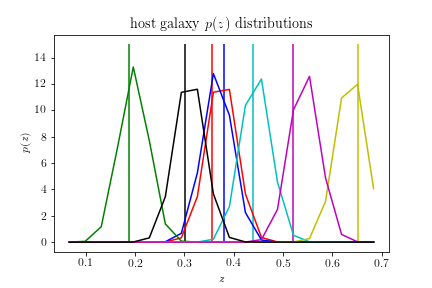
\includegraphics[width=0.5\textwidth]{fig/host_likelihoods.png}
		\caption{These are examples of mock photo-$z$ posteriors.  \textbf{(@aimalz Change these to plot as piecewise constant.)}}
		\label{fig:pzs}
	\end{center}
\end{figure}

The first term is more challenging due to its higher dimensionality.  We are modeling the expected product of a probabilistic lightcurve fitter that gives a joint probability distribution over supernova type, redshift, and distance modulus.  As this is an emulation procedure, rather than a simulation, we construct the desired quantity using an understanding of how a lightcurve fitter works.  Depending on the type of supernova, a different fitting function is used, so typically a classifier is run on the lightcurves first, and then that information is fed into a lightcurve fitter.  This is equivalent to
\begin{align}
\label{eq:lc_fit_model}
p(\mu_{n}, z_{n}, t_{n} | \mu'_{n}, z'_{n}, t'_{n}) &= p(t_{n} | t'_{n})\ p(\mu_{n}, z_{n} | \mu'_{n}, z'_{n}, t'_{n}, t_{n}).
\end{align}

The quantity $p(t | t'_{n})$ is a vector of length $T$ in which each cell is the probability of a supernova's classified type given its true type, evaluated at the true type $t'_{n}$ of supernova $n$.  The $T\times T$ matrix defined by $p(t | t')$ is called the confusion matrix $\textul{C}$ of a classifier, whose diagonal elements give the fraction of supernovae classified as their true type.  \textbf{(We need to choose a confusion matrix typical of a modern classifier and use that in the tests.)}

We motivate the mechanism producing $p(\mu_{n}, z_{n} | \mu'_{n}, z'_{n}, t'_{n}, t_{n})$.  We currently assume that this function is separable into a redshift-dependent component $p(z_{n} | z'_{n})$ and a redshift-independent component $p(\mu_{n} | \mu'_{n}, t'_{n}, t_{n})$.  \textbf{(We can and should revise this assumption.  @reneehlozek Where can we find information upon which to base a better emulation model?)}  For these, we use the same model as for the redshift posteriors based on host galaxy photometry, with a variance $\sigma_{\ell}^{2}$ and mean $z_{n}''^{\ell}$, yielding a vector of length $J$.

When constructing a traditional Hubble diagram, we only attempt to estimate a distance modulus for type Ia supernovae, leaving the distance modulus of non-standardizable types unconstrained.  This choice is based on the classified type $t_{n}$ rather than the true type.  When there is a misclassification, i.e. $t_{n}\neq t'_{n}$, a type Ia supernova might be given an unconstrained distance modulus and a core-collapse supernova would be assigned systematically incorrect distance modulus.  In particular, type II contaminants tend to have a high scatter around a constant distance modulus and type Ibc contaminants tend to be systematically biased to lower distance moduli.  \textbf{(We need to find one of those figures showing these functions!)}  Based on these observations, we establish functions $p(\mu_{n} | \mu'_{n}, t'_{n}, t_{n})$ corresponding to all elements of the confusion matrix and evaluate them at the known values of $\mu'_{n}$ and $t'_{n}$ and each possible value of $t_{n}$, yielding a $T\times K$ matrix for each supernova in the sample.  The functions used in this emulation procedure are as follows
\begin{align}
\label{eq:emulation}
p(\mu_{n} | \mu'_{n}, t'_{n}=Ia, t_{n}=Ia) &= \mathcal{N}(\mu''_{n}, \sigma_{Ia}^{2})\ with\ \mu''_{n}\sim\mathcal{N}(\mu'_{n}, \sigma_{Ia}^{2})\\
p(\mu_{n} | \mu'_{n}, t'_{n}=Ibc, t_{n}=Ia) &= \mathcal{N}(\mu''_{n}, \sigma_{Ibc}^{2})\ with\ \mu''_{n}\sim\mathcal{N}(\mu'_{n} - c_{Ibc}, \sigma_{Ibc}^{2})\\
p(\mu_{n} | \mu'_{n}, t'_{n}=II, t_{n}=Ia) &= \mathcal{N}(\mu''_{n}, \sigma_{II}^{2})\ with\ \mu''_{n}\sim\mathcal{N}(c_{II}, \sigma_{II}^{2})\\
p(\mu_{n} | \mu'_{n}, t'_{n}, t_{n}\neq Ia) &= U(\mu_{min}, \mu_{max}),
\end{align}
where $c_{Ibc}$ and $c_{II}$ are constants shared among all supernovae.

\subsubsection{Incorporating the selection function}
\label{sec:selectionfunctions}

So far, we have not considered the effect of selection functions in the space of observed supernova lightcurves and host galaxy photometry, though they are obviously very important.  We assume that the survey producing the catalog of three-dimensional posteriors knows its selection functions in the space of data, which correspond to $p(\textul{\ell} | \vec{\alpha})$ and $p(\vec{f} | \vec{\beta})$.  Given models for the relationships between data and latent variables $p(\mu, z, t | \textul{\ell})$ and $p(z | \vec{f})$, we could marginalize over the space of all possible data to obtain $p(\mu, z, t | \vec{\alpha})$ and $p(z | \vec{\beta})$, which would then simply be multiplied to get $p(\mu, z, t | \vec{\alpha}, \vec{\beta})$.  

Because we do not simulate the supernova lightcurves nor host galaxy photometry, this approach is not available to us.  Once again, we will emulate it, this time using summary statistics of mock data from realistic simulations.  We can calculate the recovery rate in the space of latent variables given different selection function parameters by actually imposing those selection functions on realistic simulations for which the true distribution in the space of $\mu$, $z$, and $t$ is known. 

In the simple case of host galaxy photometry, we assume the cuts in magnitude and signal-to-noise ratio expected of LSST and apply these to the photometry of the Buzzard catalog with a known redshift distribution.  By simply taking the ratio of recovered galaxies to simulated galaxies within each of the $J$ redshift bins.  Note that we have already assumed no correlation between host galaxy properties and supernova type, but if there were a simulation that accurately included this effect, we could obtain a selection function in the space of $t$ and $z$ based on that.  \textbf{(We need to actually do this with realistic cuts and mock data.)}  This procedure gives us $p(z | \vec{\beta})$.

In the three-dimensional case of supernova lightcurves, there is not a mock dataset with information on the true number of supernovae at each $\mu$, $z$, and $t$.  \textbf{(Is this the nominal reason why we have to take the ratio of what's recovered with the WFD selection cuts to what's recovered with the DDF selection cuts?  I don't understand how we have either of those numbers if that data is not available.  Is it because the recovery rate requires choosing a classifier and lightcurve fitter?)}  Instead of using the ratio of the number of supernovae recovered over the number of supernovae simulated as a function of their latent variables, we use the ratio of the recovery rate for the selection function in question over the recovery rate for the most generous possible selection function.  For LSST, these correspond to the Wide Fast Deep (WFD) and Deep Drilling Fields (DDF) selection functions.  This procedure gives us $p(\mu, z, t | \vec{\alpha})$.

\subsubsection{Making interim posteriors}
\label{sec:interimpriors}



To make interim posteriors, we introduce the interim priors of Eq. \ref{eq:second}.  We choose $\vec{\theta}^{*}$ and $\textul{\phi}^{*}$ [specify what a good, general choice would be].  Because the parametrization hasn't changed, the term $p(z_{\zeta}, t_{\tau} | \textul{\phi}^{*})$ takes the simple form of $\phi^{*}_{\tau\zeta}$.  Similarly, $p(\mu_{\nu} | z_{\zeta}, \vec{\theta}^{*})$ will be a delta function $\delta_{f_{\vec{\theta}^{*}}(z_{\zeta})}(\mu_{\nu})$.  

Finally, in Eq \ref{eq:interimposteriordata}, we put these pieces together to express the form of the individual interim posteriors of the form of Eq. \ref{eq:mockBayes}.

\begin{align}
\label{eq:interimposteriordata}
p_{n}(\mu_{\nu}, z_{\zeta}, t_{\tau} | \textul{\ell}_{n}, \vec{m}_{n}, \vec{\theta}^{*}, \textul{\phi}^{*}) &= KC_{\tau'_{n}\tau}\mathcal{N}_{(\hat{z}^{\ell}, \hat{\mu}^{\ell}), \textul{\Sigma}_{n}}(z_{\zeta}, \mu_{\nu}) \mathcal{N}_{\hat{z}_{n}^{m}, \sigma_{n}^{2}}(z_{\zeta}) \phi^{*}_{\zeta\tau}\delta_{f_{\vec{\theta}^{*}}(z_{\zeta})}(\mu_{\nu})
\end{align}

The constant of proportionality $K$ here will be set such that $\sum_{\nu}^{D}\sum_{\zeta}^{Z}\sum_{\tau}^{T} p_{n}(\mu_{\nu}, z_{\zeta}, t_{\tau} | \textul{\ell}_{n}, \vec{m}_{n}, \vec{\theta}^{*}, \textul{\phi}^{*})=1$.



\section{Validation}

%\clearpage
%
%\begin{itemize}
%\item $p(z_{n}, t_{n} | \textul{\phi}^{*})$: 
%\item $p(\mu_{n} | z_{n}, \vec{\theta}^{*})$
%\item $p(\vec{m}_{n} | \mu_{n}, z_{n})$
%\item $p(\textul{\ell}_{n} | \mu_{n}, z_{n}, t_{n})$
%\end{itemize}
%
%We will first draw pairs of true parameters $(T_{n}^{0}, z_{n}^{0})$ from $p(T_{n}, z_{n} | \textul{\Phi}_{0}) = \mathcal{D}\left[\textul{\Phi}_{0}\right]$, which in this case is a discrete distribution.  Then we will calculate the true $\mu_{n}^{0}$ according to [insert distance modulus equation here] from $z_{n}^{0}$ and $\vec{\theta}_{0}$.  This may be interpreted as $p(\mu_{n} | z_{n}, \vec{\theta}) = 1$, so $p(\mu_{n}, z_{n}, T_{n} | \vec{\theta}^{*}, \textul{\Phi}^{*}) = p(z_{n}, T_{n} | \textul{\Phi}^{*}) p(\mu_{n} | z_{n}, \vec{\theta}^{*})$
%
%Next, we will construct three-dimensional likelihoods for each supernova over $\mu_{n}$, $z_{n}$, and $T_{n}$.  $\textul{\ell}_{n}$ and $\vec{f}_{n}$ are independent of one another, so we may state Eq. \ref{eq:independentdata}.
%
%\begin{align}
%\label{eq:independentdata}
%p(\textul{\ell}_{n}, \vec{f}_{n} | \mu_{n}, z_{n}, T_{n}, \vec{\theta}^{*}, \textul{\Phi}^{*})\ p(\mu_{n}, z_{n}, T_{n} | \vec{\theta}^{*}, \textul{\Phi}^{*})
%\end{align}
%
%We know $p(T_{n} | T_{n}^{0})$ as the row $\vec{r}(T_{n}^{0}) = p(T_{n} | T_{n}^{0})$ of the confusion matrix corresponding to $T_{n}^{0}$.  We denote this as the discrete distribution $p(T_{n} | T_{n}^{0}) = \mathcal{D}\left[\vec{r}(T_{n}^{0})\right]$.  In the simplest case, the redshifts are Gaussian distributions of variance $\sigma_{z}^{2}$ about $z_{n}' \sim \mathcal{N}\left[z_{n}^{0}, \sigma_{z}^{2}\right]$ for a constant $\sigma_{z}$ across the whole survey.  Thus we may write $p(z_{n} | z_{n}^{0}) = \mathcal{N}\left[z_{n}', \sigma_{z}^{2}\right]$ and $p(z_{n}, T_{n} | z_{n}^{0}, T_{n}^{0}) = p(z_{n} | z_{n}^{0}) p(T_{n} | T_{n}^{0})$.
%
%We know that $p(\mu_{n} | T_{n}, z_{n})$ will be nontrivial because 
%
%\begin{align}
%T_{n}' &\sim D[\vec{r}(T_{n})]\\
%z_{n}' &\sim \vec{\Phi}(T_{n})\\
%\mu_{n}' &= \mu(z_{n}', \vec{\theta})
%\end{align}

\section{Discussion}

\section{Conclusion}

%\acknowledgments

%\appendix

\bibliography{references}

\end{document}